\section{{\tt burn\_cell}}

\subsection{Getting Started}

The {\tt burn\_cell} codes are located in {\tt Microphysics/unit\_test/burn\_cell}. To run a simulation, ensure that both an input file and an initial conditions file have been created and are in the same directory as the executable. 

\subsection{Input File}

These files are typically named as {\tt inputs\_burn\_network} where {\tt network} is the network you wish to use for your testing.

This structure of this file is is fairly self-explanitory.
The run prefix defined should be unique to the tests that will be run as they will be used to identify all of the output files. Typically, the run prefix involves the name of the network being tested. 
The {\tt atol} variables define absolute tolerances and the {\tt rtol} variables define the relative tolerances. 

\subsection{Initialization File}

These files are normally named as {\tt init\_network} where {\tt network} is the network used for testing. 
It collects all of the inputs that {\tt main.f90} asks for onto individual lines of a file so that the user does not have to input all 5$+$ parameters that are required everytime the test is run. 
The use of each line is defined in Table~\ref{tab:init-structure}.

\begin{table}
	\centering
	\begin{tabular}{|l|l|l|}
		\hline
			\multicolumn{1}{|c|}{\textbf{Line}} &
			\multicolumn{1}{|c|}{\textbf{Name in {\tt main.f90}}} &
			\multicolumn{1}{|c|}{\textbf{Definition}} \\
		\hline
		\rowcolor{tableShade}
		1 & {\tt tmax} & Maximum Time (s) \\
		2 & {\tt ntimes} & Number of time subdivisions \\
		\rowcolor{tableShade}
		3 & {\tt burn\_state\_in\%rho} & State Density ($\frac{g}{cm^3}$) \\
		4 & {\tt burn\_state\_in\%T} & State Temperature (K) \\
		\rowcolor{tableShade}
		5, 6, 7, ... & {\tt burn\_state\_in\%xn(i)} & Mass Fractions \\
		\hline
	\end{tabular}
	\caption{The structure of the init\_network files used in {\tt main.f90}.}
	\label{tab:init-structure}
\end{table}

\subsection{Running the Code}

To run the code, enter the {\tt burn\_cell} directory and run {\tt ./main.Linux.gfortran.exe} where the first argument is the inputs file and then the lines from the initial conditions file are redirected into the code using {\tt <}. 
For example: {\tt ./main.Linux.gfortran.exe inputs\_burn\_aprox13 < init\_aprox13}

For however many events are run, defined as { \tt ntimes} in the initial conditions file, the code will output that many files into the present working directory. 
They will be named using the run prefix definied in the inputs file.

Next, run {\tt burn\_cell.py} using Python3 and listing the defined run prefix as an argument.
For example: {\tt python3 burn\_cell.py react\_aprox13}. 
The burn\_cell code will gather information from all of the output files and compile them into three graphs explained below.

Once finished, the user can clear up their directory by removing all of the main output files: {\tt rm -rf runprefix\_0*}. 
Be careful not to forget the first 0 or all of the graphs will be deleted as well. 
Or, to save the data, create a new directory and move all of the output files there. 

\subsection{Graphs Output by burn\_cell.py}

The file {\tt run-prefix\_logX.png} and {\tt run-prefix\_logX.eps} will display a graph of the chemical abundances as a function of the time, both on logarithmic scales, for all species involved in the simulation. 
An example of this graph is shown in Figure~\ref{fig:aprox13_logX}.

\begin{figure}
        \centering
	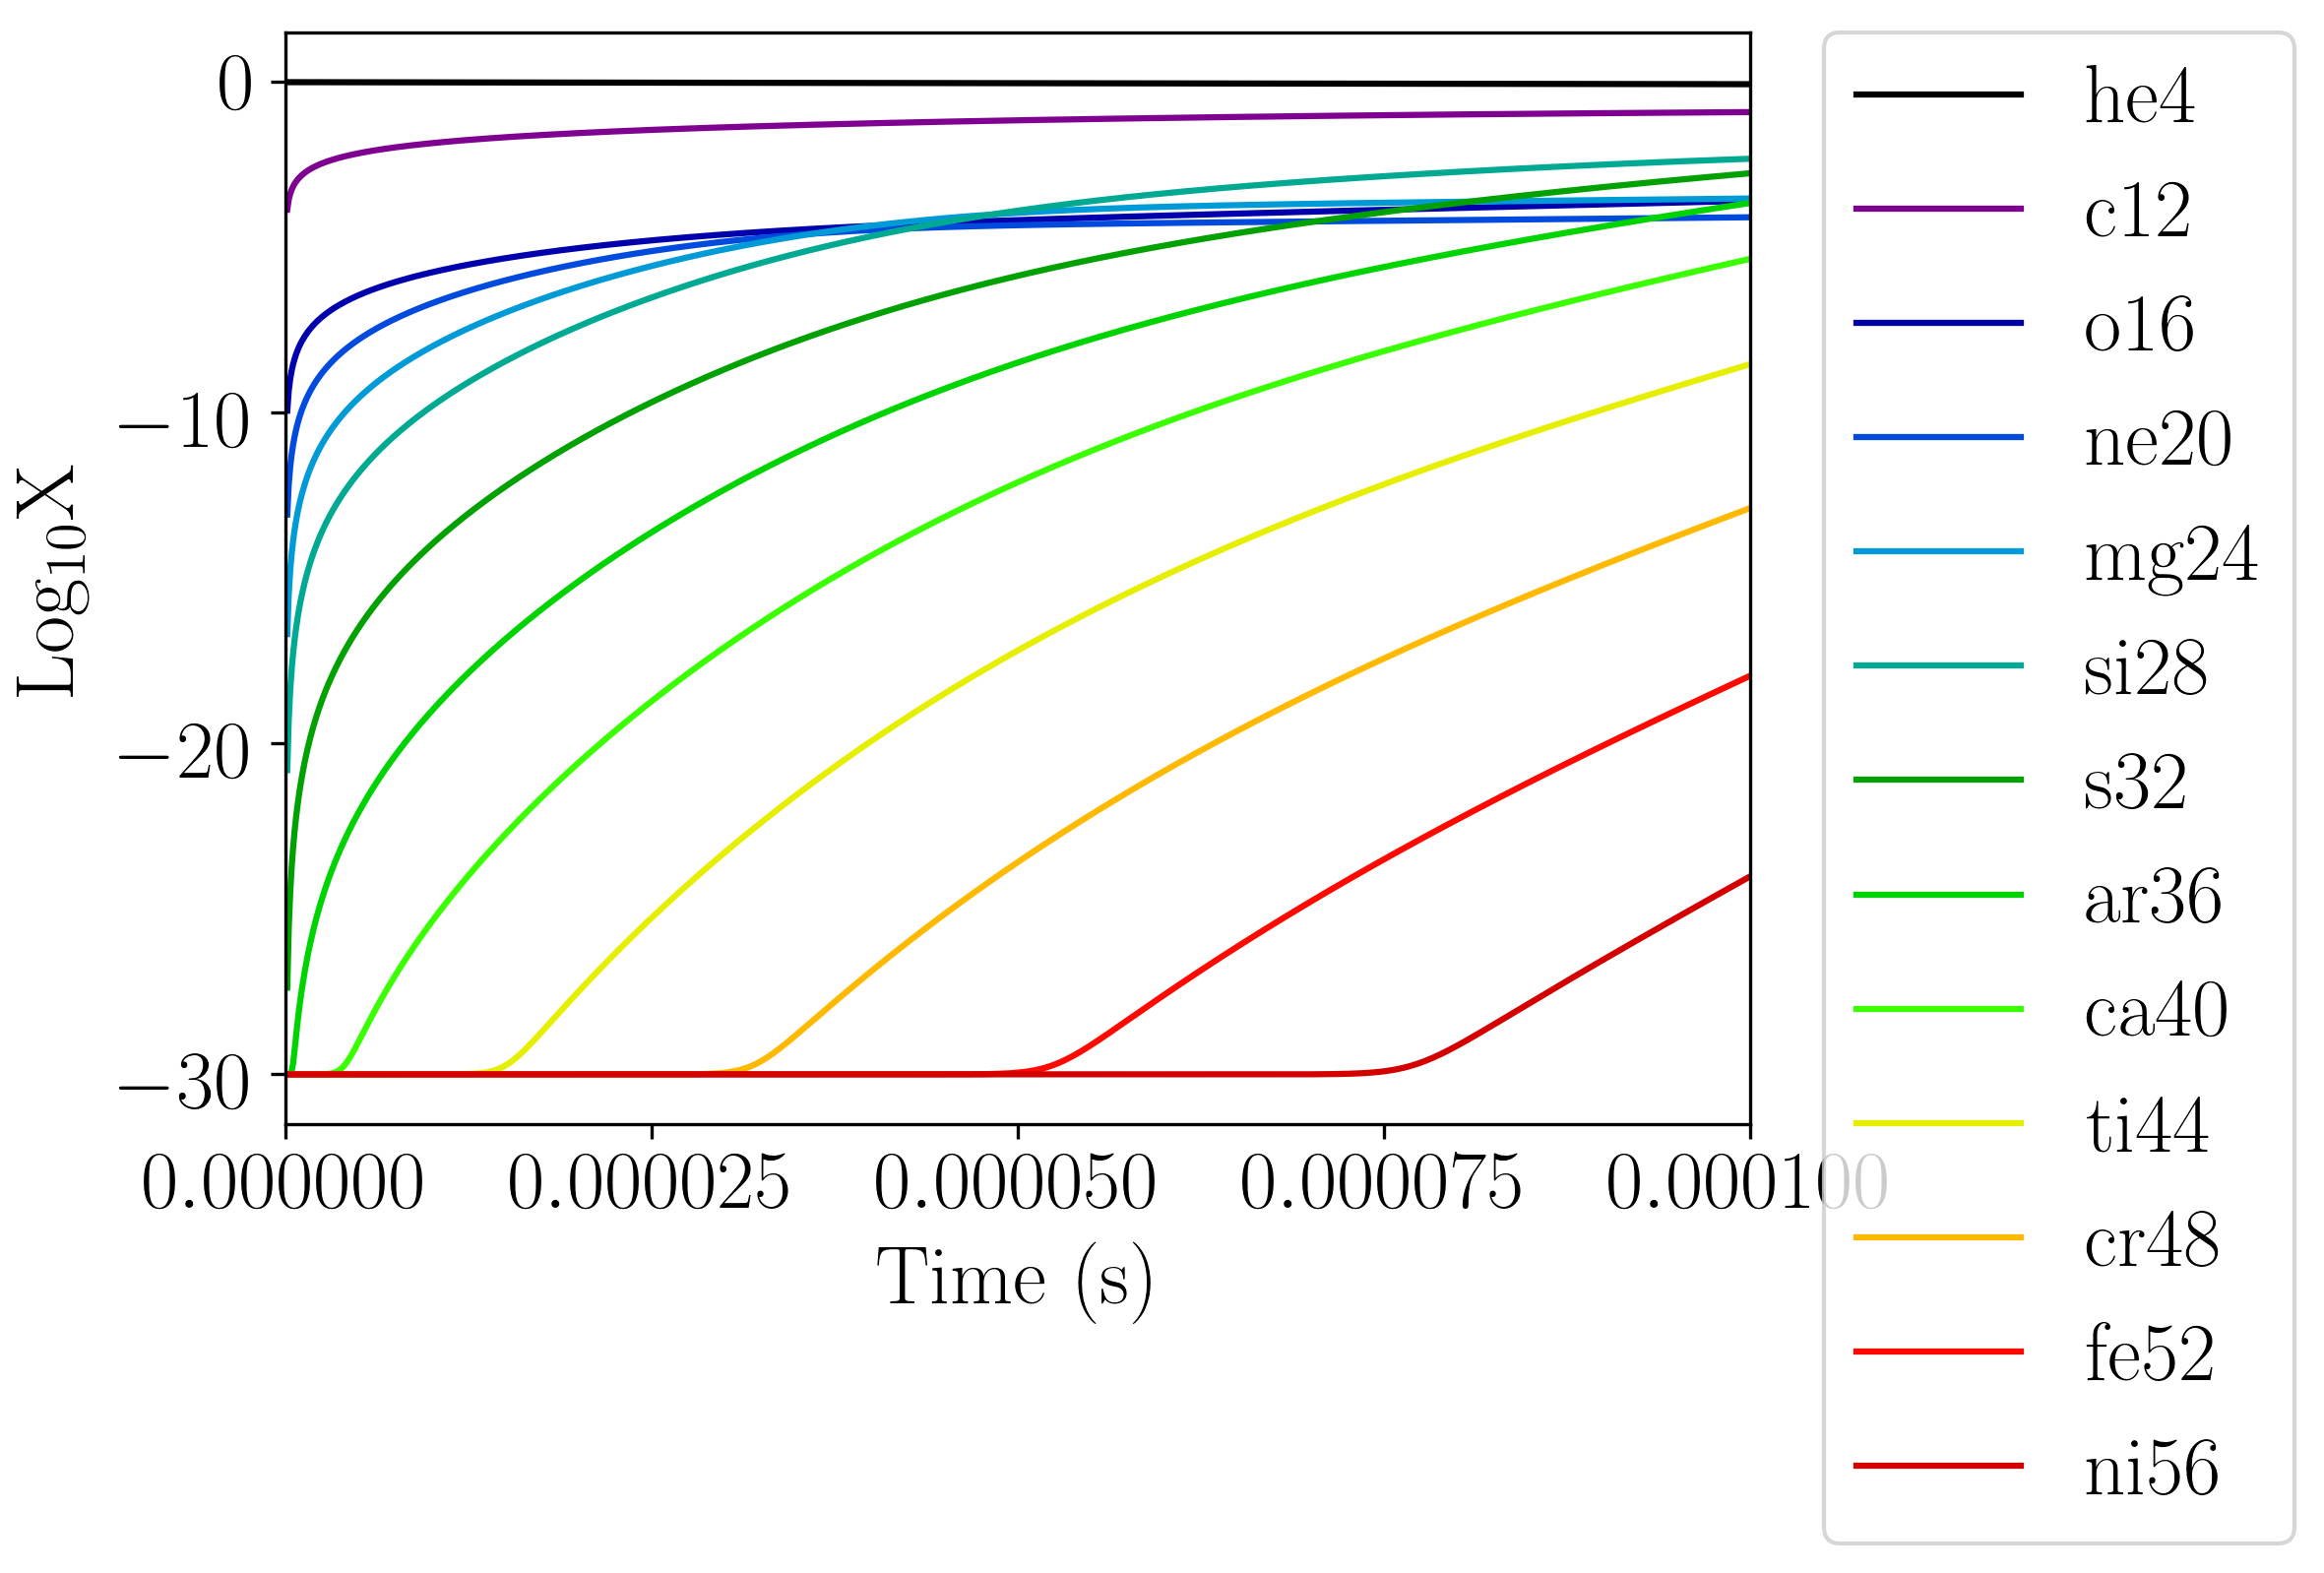
\includegraphics[width=4.5in]{react_aprox13_logX}
	\caption{An example of a plot output by the {\tt burn\_cell} unit test. This is the { \tt logX } output cooresponding to the network { \tt aprox13}.}
	\label{fig:aprox13_logX}
\end{figure}

The file {\tt run-prefix\_ydot.png} and {\tt run-prefix\_ydot.eps} will display the Moller fraction (mass fraction / atomic weight) as a function of time, both on logarithmic scales, for all species involved in the code. 

The file {\tt run-prefix\_T-edot.png} and {\tt run-prefix\_T-edot.eps} will display the Temperature and the Energy Generation Rate as a function of time. 
